\documentclass[12pt]{article}

\usepackage{sbc-template}

\usepackage{float}

\usepackage[table]{xcolor}

\usepackage{graphicx,url}

\usepackage[brazil]{babel}

\usepackage[utf8]{inputenc}  

     
\sloppy

\title{Telemetria do jogo eletrônico Forza Horizon 5 com o microcontrolador ESP32 e um display LCD 16x2}

\author{João Pedro Pereira Lemos\inst{1}}


\address{
  Instituto Federal de Educação, Ciência e Tecnologia do Estado do Ceará (IFCE)
  \email{joao.pedro.pereira62@aluno.ifce.edu.br}
}

\begin{document}

\maketitle

\begin{abstract}
  This project aims to obtain telemetry information from the Forza Horizon 5 video game
  from the UDP protocol, using the ESP32 microcontroller, and display it using a 16x2 display.
\end{abstract}

\begin{resumo}
  Este projeto tem por objetivo obter as informações de telemetria do jogo eletrônico
  Forza Horizon 5 a partir do protocolo UDP, utilizando o microcontrolador ESP32,
  e realizar sua exibição utilizando um display 16x2.
\end{resumo}

\section{Introdução}

A interconexão de dispositivos físicos com capacidades computacionais de detecção e comunicação
de dados é denominada internet das coisas, ou IoT, em inglês. Hoje, se observa um crescente número
de dispositivos conectados à internet, e com eles, a criação de um ecossistema completo.
Esses microcontroladores possuem uma  gama de aplicações, que vão desde automações simples,
até grandes projetos~\cite{carrion}.

Hoje, com a popularização de diversos microcontroladores, é comum que pessoas interessadas desenvolvam
os mais diversos tipos de projetos, que envolvam tecnologias sem fio, como Wi-Fi e Bluetooth.
A comunidade denomina esses projetos como parte da chamada cultura “maker”.
Muitos desses projetos são criados com o propósito de educar, demonstrar um conceito, ou mesmo por hobby~\cite{gavassa}.

O presente trabalho utiliza o microcontrolador ESP32 em conjunto com um display LCD de 16 colunas e 2 linhas,
para realizar o monitoramento da telemetria proveniente do jogo eletrônico intitulado Forza Horizon 5, no sistema Windows 10.
O jogo envia os dados pela rede, utilizando o protocolo UDP, e a plataforma do ESP32 realiza a decodificação de tais dados
e os exibe no display LCD, utilizando o protocolo I2C.
Os dados são atualizados em tempo real, conforme são emitidos pelo jogo.

\section{Fundamentação teórica}

Projetos modernos de IoT são criados com diversos microcontroladores. Dentre estes dispositivos, destaca-se o ESP32.
Este microcontrolador foi projetado pela Espressif Systems, no ano de 2016.
Suas principais características são a velocidade de processamento, acessibilidade e conectividade.
Este microcontrolador suporta as tecnologias Wi-Fi e Bluetooth nativamente, sem a necessidade de utilizar módulos externos.
Assim, é comum encontrar projetos criados com este microcontrolador que acessam servidores remotos, APIs de terceiros,
ou mesmo que são capazes de criar um próprio servidor local~\cite{kolban}.

Este poderoso microcontrolador é capaz de utilizar protocolos de comunicação sem fio, como o
TCP (Protocolo de Controle de Transmissão, em português) e UDP (Protocolo de Datagrama do Usuário, em português).
Em~\cite{jesus-junior}, foi desenvolvido um sistema de aquisição de dados de extensometria aplicado a um tambor
descascador de toras de madeira, em que é utilizado o microcontrolador ESP32, e o protocolo UDP foi escolhido em
detrimento do TCP, por questões de velocidade. Neste sistema, o microcontrolador ESP32 envia um pacote de dados
via UDP a um outro ESP32 servidor, que é conectado à porta USB de um computador, realizando a aquisição dos dados.

O jogo eletrônico Forza Horizon 5, lançado em 2021 por Xbox Game Studios e desenvolvido pela Playground Games,
é um jogo automobilístico que mistura a experiência de jogos arcade casuais com as mecânicas realistas dos jogos simuladores.
É possível, por exemplo, ajustar a pressão dos pneus, transmissão, molas e válvulas do veículo, dentre outras customizações.

O jogo permite a integração com alguns dispositivos, como volantes, câmbios e pedais, além de painéis que exibem em tempo
real as informações sobre o veículo.
Para isso, faz uso de uma conexão com o protocolo UDP, onde envia bytes com a telemetria do jogo para o dispositivo alvo.
Existem alguns projetos de código aberto que conseguem decodificar e interpretar corretamente os dados da telemetria,
como o projeto intitulado “forza-telemetry” de Austin Baccus, disponível na plataforma GitHub~\cite{baccus}.

\section{Materiais e métodos}

Para realizar este projeto, foram utilizados alguns materiais. Utilizou-se o microcontrolador ESP32,
juntamente de um display LCD de 16 colunas e duas linhas, com suporte ao protocolo I2C.
Este microcontrolador é alimentado via cabo, no padrão micro-USB.
Para executar o jogo eletrônico Forza Horizon 5, utilizou-se um computador com configurações adequadas.
A figura~\ref{fig:illustration} ilustra de forma simplificada o funcionamento do projeto.

\begin{figure}[ht]
  \centering
  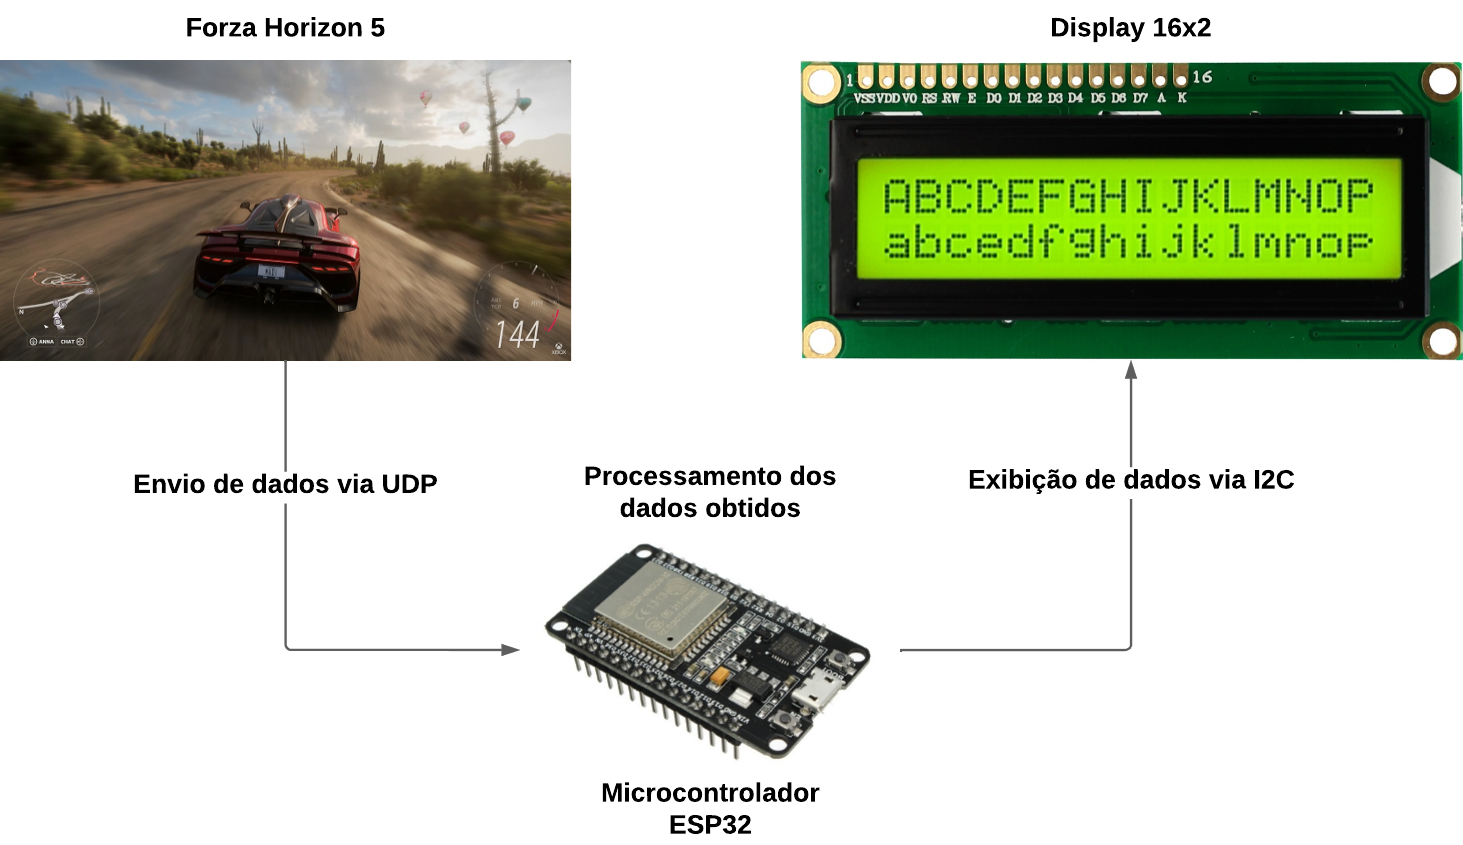
\includegraphics[width=0.9\textwidth]{images/illustration.png}
  \caption{Ilustração do projeto}
  \label{fig:illustration}
\end{figure}

\subsection{Microcontrolador ESP32}

O ESP32 é um módulo de alta performance para aplicações envolvendo Wi-Fi, contando com um baixíssimo consumo de energia.
É uma evolução do já conhecido ESP8266, com maior poder de processamento e Bluetooth BLE 4.2 embutido.
Na placa temos o chip ESP32 da Espressif, com antena embutida, uma interface USB-Serial e um regulador de tensão de 3.3V.
A programação pode ser feita utilizando a linguagem de programação Lua, ou usando a IDE do Arduino, através de um cabo micro-usb.
O ESP32 conta com uma CPU dual-core de 32 bits, e possui um clock máximo de 240 MHz. Seu módulo Wi-Fi trabalha em 2.4 GHz,
e nos padrões 802.11 b/g/n, em até 150 Mbps. Possui 11 portas GPIO com funções de PWM, I2C, SPI, dentre outras~\cite{esp32}.

\begin{figure}[ht]
  \centering
  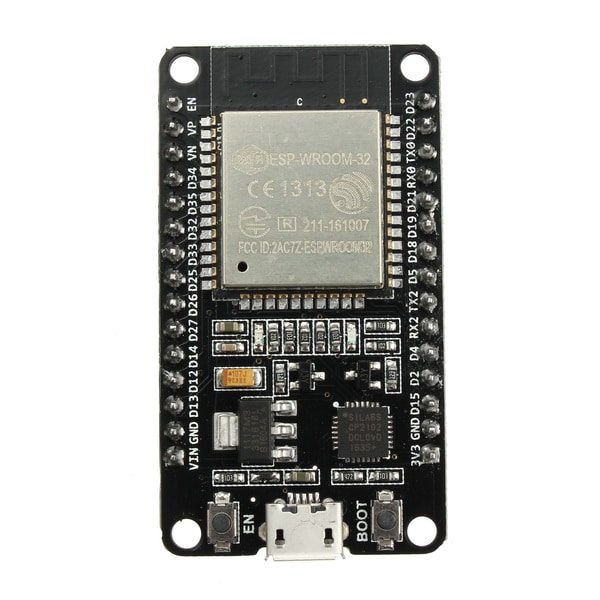
\includegraphics[width=.3\textwidth]{images/esp32.jpg}
  \caption{Microcontrolador ESP32}
  \label{fig:esp32}
\end{figure}

\subsection{Display LCD 16x2 com suporte a I2C}

Um display LCD é uma interface de comunicação visual. Utilizaremos um display de 16 colunas e 2 linhas,
e que suporta o protocolo I2C. I2C significa \emph{Inter Integrated Circuits}, ou Circuitos Inter Integrados, em português.
I2C é um protocolo de comunicação síncrona, o que significa que ambos os dispositivos que estão compartilhando as informações
devem compartilhar um sinal de clock comum. Ele tem apenas dois fios, SDA e SCL para compartilhar informações, dos quais SCL é
usado para o sinal do relógio e SDA é usado para enviar e receber dados.
O display possui um controlador HD44780~\cite{display}.

\begin{figure}[ht]
  \centering
  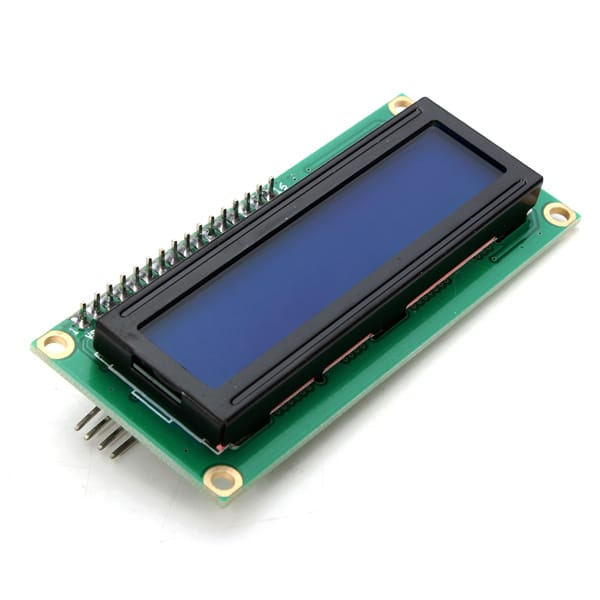
\includegraphics[width=.3\textwidth]{images/display.jpg}
  \caption{Display LCD 16x2 com suporte a I2C}
  \label{fig:display}
\end{figure}

\subsection{Funcionamento do projeto}

A seguir, vamos discorrer sobre o funcionamento deste projeto. Para que os dados do jogo possam ser exibidos no display,
foi necessário realizar a conexão do mesmo com o ESP32. O pino GND do display deve foi conectado ao pino GND do ESP32.
O pino VCC do display deve foi conectado ao pino 3V3 do ESP32. O pino SDA do display foi ser conectado ao pino
D21 do ESP32. O pino SCL do display foi ser conectado ao pino D22 do ESP32.
A figura~\ref{fig:schematic} ilustra tais conexões.

\begin{figure}[ht]
  \centering
  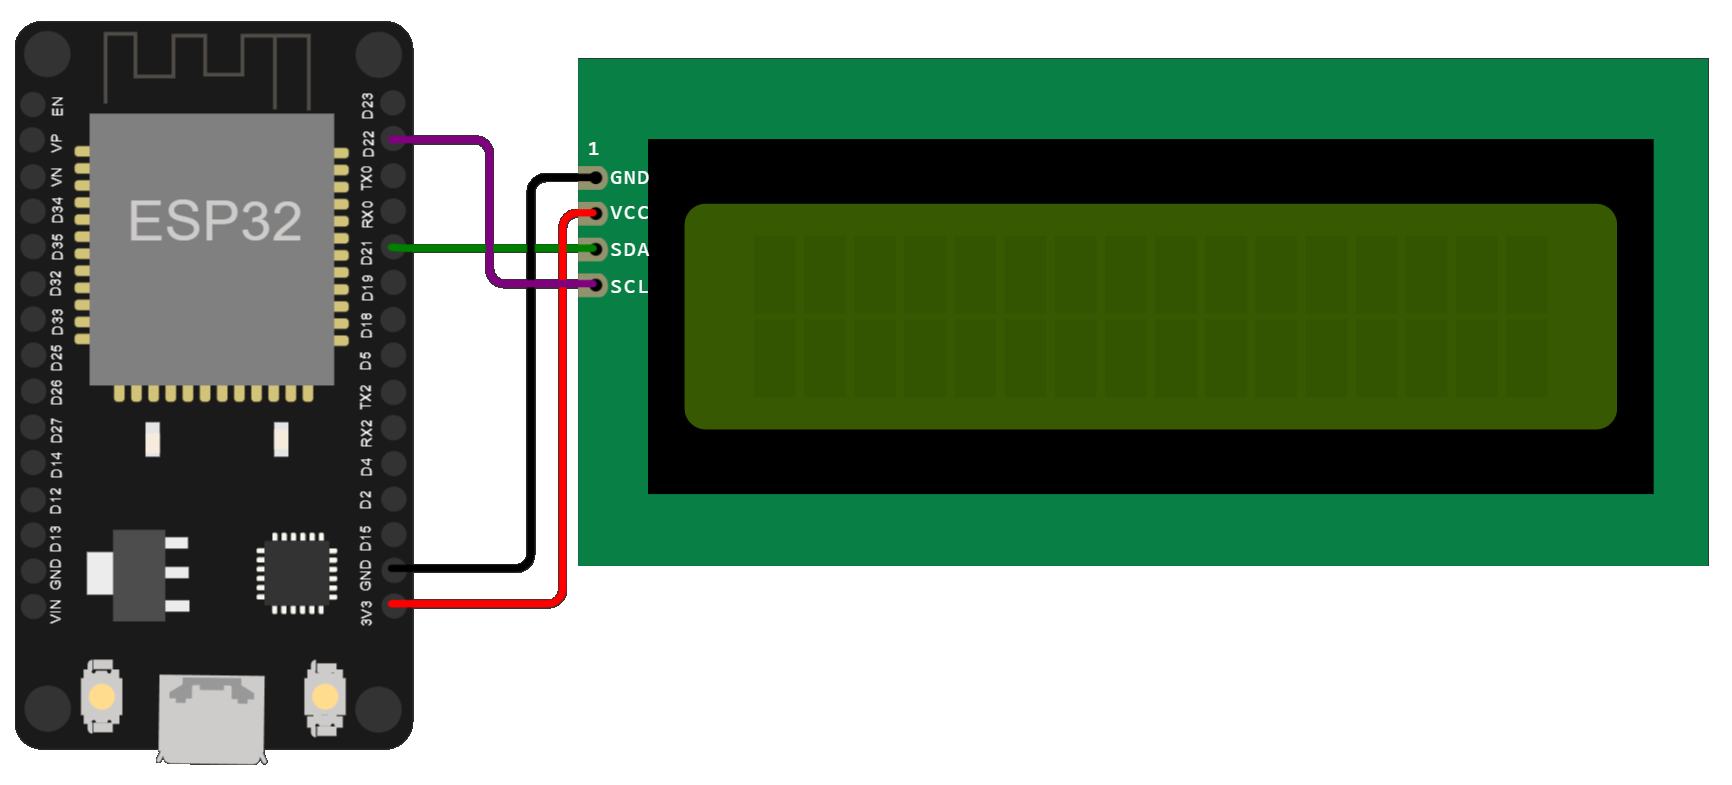
\includegraphics[width=.7\textwidth]{images/schematic.png}
  \caption{Esquemático do projeto}
  \label{fig:schematic}
\end{figure}

Após realizar as conexões físicas, foi necessário conectar o ESP32 à mesma rede local em que o computador que executa o jogo
está conectado. Para isso, utilizamos o módulo Wi-Fi do ESP32. Assim que a conexão é estabelecida, o ESP32 exibe o IP local
adquirido, por meio do display, conforme a figura~\ref{fig:connected}.
De posse do IP, configuramos então o Forza Horizon 5 para enviar os dados de telemetria no endereço e portas indicados,
conforme a figura~\ref{fig:forza_settings}.

\begin{figure}[ht]
  \centering
  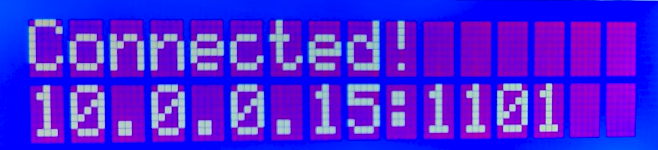
\includegraphics[width=.7\textwidth]{images/connected.png}
  \caption{ESP32 conectado à rede local}
  \label{fig:connected}
\end{figure}

\begin{figure}[ht]
  \centering
  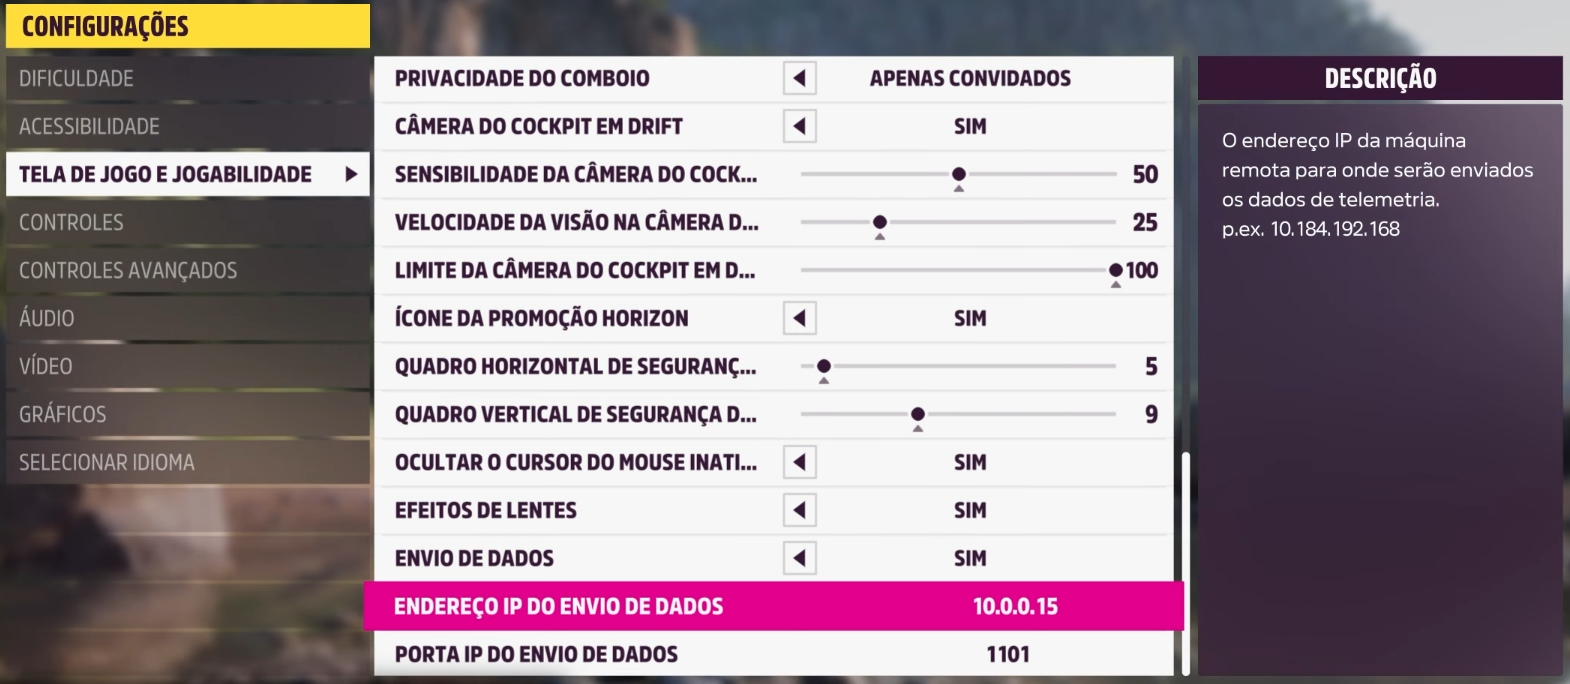
\includegraphics[width=.7\textwidth]{images/forza_settings.png}
  \caption{Configurações do Forza Horizon 5}
  \label{fig:forza_settings}
\end{figure}

Deste ponto em diante, ESP32 recebe os dados do jogo, e realiza a decodificação apropriada dos pacotes UDP.
Os dados decodificados são: velocidade do veículo, rotações por minuto do motor do veículo, marcha atual,
e caso o jogador esteja em um evento do jogo, a posição atual do veículo na corrida.
Caso o jogador esteja em um menu do jogo ou em uma tela de carregamento, uma mensagem informando que o jogo
não está em execução é exibida.
A figura~\ref{fig:project_fluxogram} apresenta um fluxograma do funcionamento do projeto.

\begin{figure}[ht]
  \centering
  \includegraphics[width=1\textwidth]{images/project_fluxogram.png}
  \caption{Fluxograma do projeto}
  \label{fig:project_fluxogram}
\end{figure}

\subsection{Metodologia de desenvolvimento}

Inicialmente, foi realizada uma  investigação sobre o funcionamento da telemetria no jogo Forza Horizon 5,
de modo a entender suas capacidades e limitações, bem como entender a estrutura dos dados que o jogo envia, e
como realizar a sua decodificação de maneira apropriada.

Logo em seguida, foi averiguado o funcionamento do protocolo UDP no ESP32.
Então, iniciou-se uma pesquisa sobre a exibição dos dados em um display 16x2. A decisão de utilizar
o protocolo I2C surgiu a partir desta pesquisa, visto que a utilização de um display sem utilizar este protocolo
seria mais complexa, além de requerer o uso de um potenciômetro para regular o contraste do display.

Finalmente, a implementação e gravação do firmware no ESP32 foi realizada, e os seus resultados, coletados.
O firmware foi escrito utilizando o editor de código gratuito Visual Studio Code, que é de código aberto e conta
com um suporte a extensões. Dentre elas, foi utilizada a extensão do PlatformIO, que nos fornece um arcabouço para o
desenvolvimento na plataforma do ESP32.
O firmware foi escrito na linguagem C++, é de código aberto e está disponível para consulta~\cite{forza-monitor, vscode, platformio}.

De posse dos dados, iniciou-se a etapa de análise dos resultados e
a escrita deste artigo. A figura~\ref{fig:development_fluxogram} mostra as etapas de forma resumida.

\begin{figure}[ht]
  \centering
  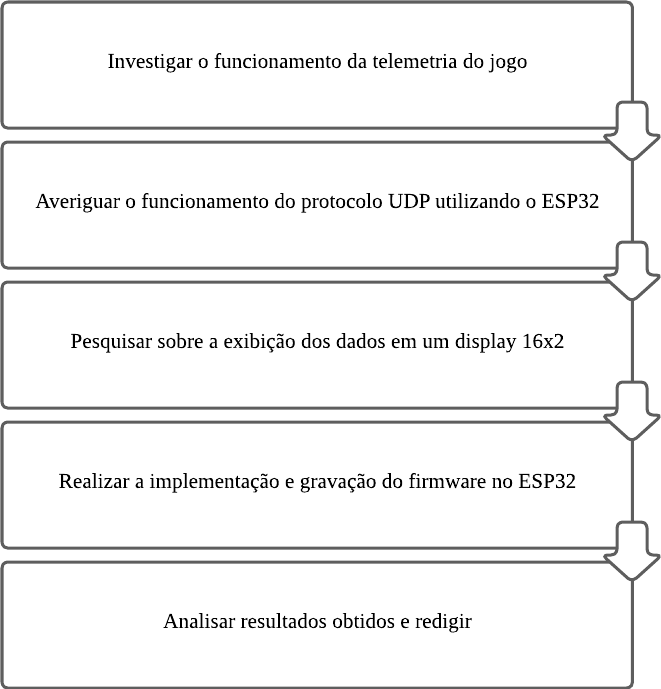
\includegraphics[width=.7\textwidth]{images/development_fluxogram.png}
  \caption{Etapas do desenvolvimento}
  \label{fig:development_fluxogram}
\end{figure}

\section{Resultados obtidos}

A seguir, temos o resultado final deste projeto.
As figuras mostram o jogo em pleno funcionamento, bem como o conteúdo
exibido pelo display 16x2. A figura~\ref{fig:real_overworld} demonstra o caso
em que o jogador está dirigindo livremente pelo mapa, sem participar de um evento.
A velocidade do veículo, a rotação do motor e a marcha atual são exibidas no display.
A figura~\ref{fig:real_on_race} demonstra o caso em que o jogador está participando de um
evento do jogo (neste caso, uma corrida de circuito).
A velocidade do veículo, a rotação do motor, a marcha atual e a posição na corrida são exibidas no display.
A figura~\ref{fig:real_menu} demonstra o caso em que o jogo está em um menu, e apenas uma mensagem
informativa é exibida no display.\clearpage

\begin{figure}[H]
  \centering
  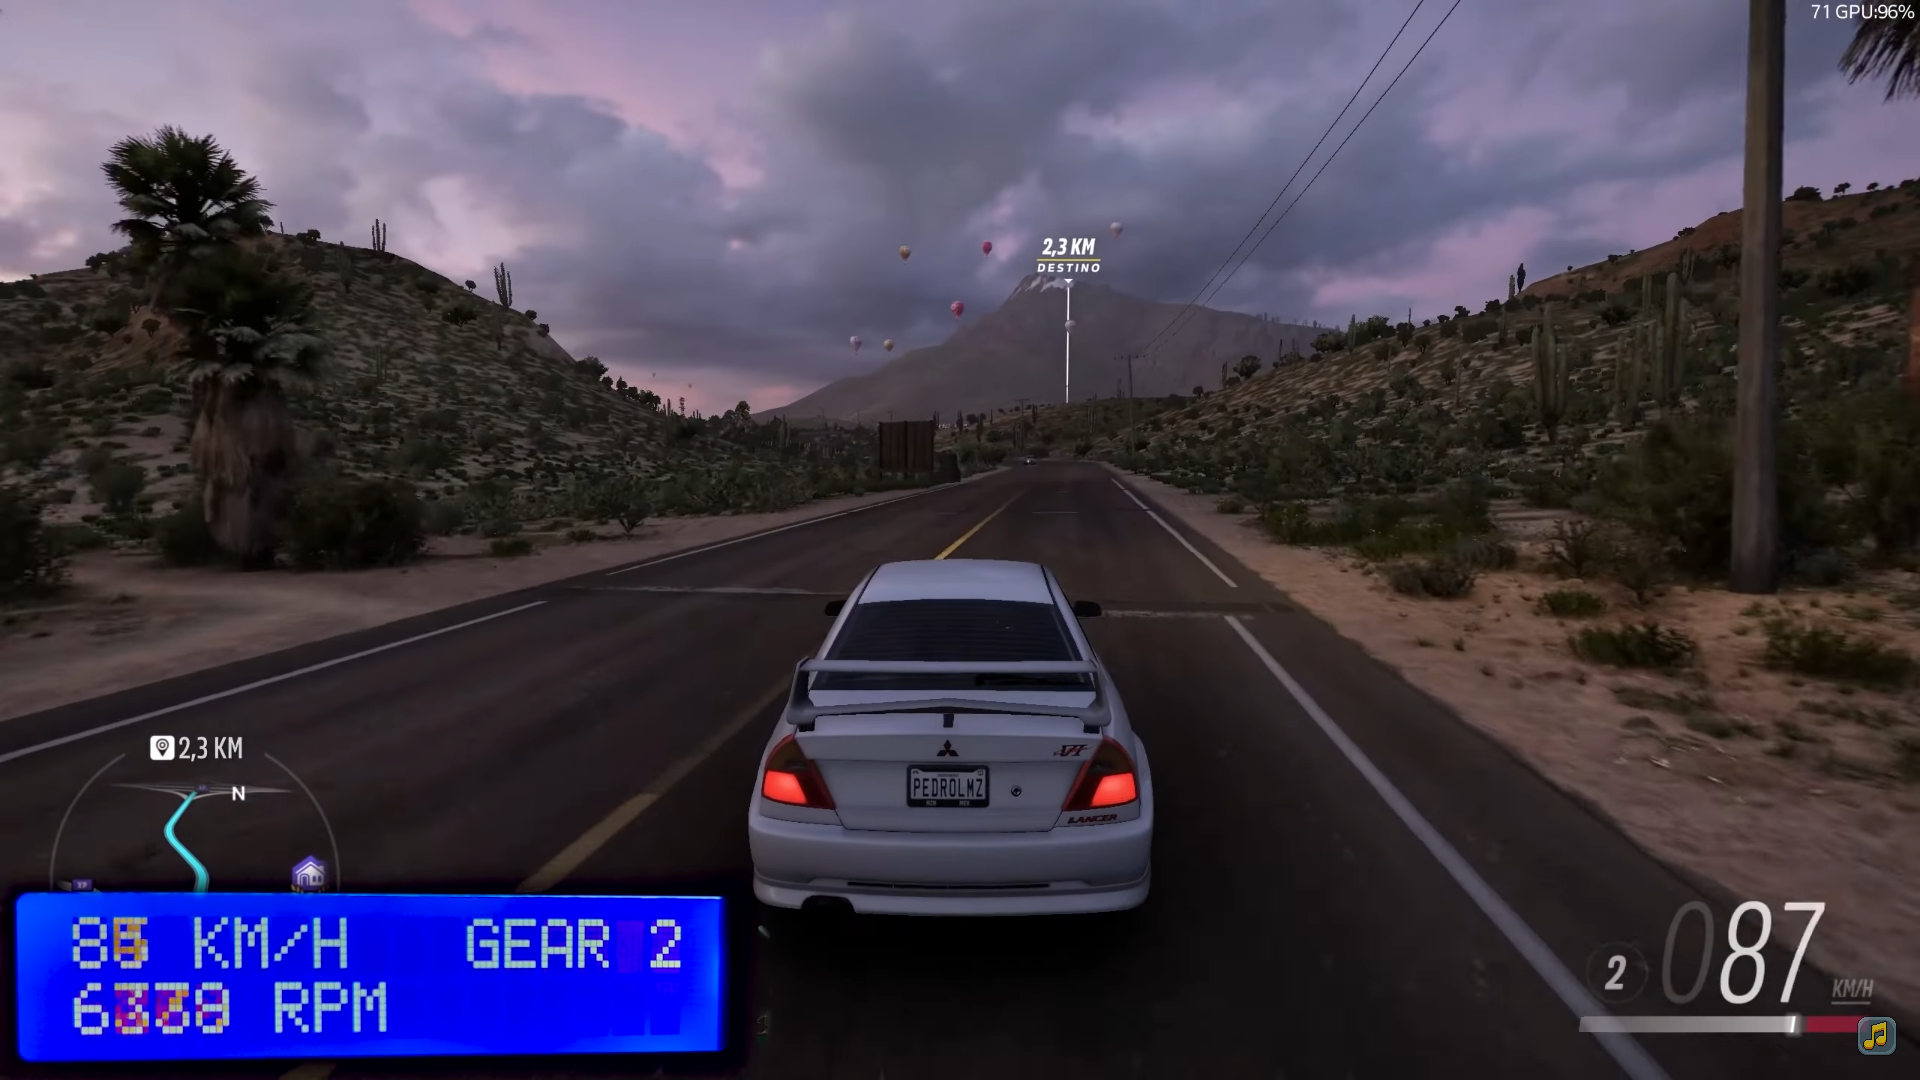
\includegraphics[width=.7\textwidth]{images/real_overworld.png}
  \caption{Exibição ao dirigir livremente}
  \bigskip
  \label{fig:real_overworld}
  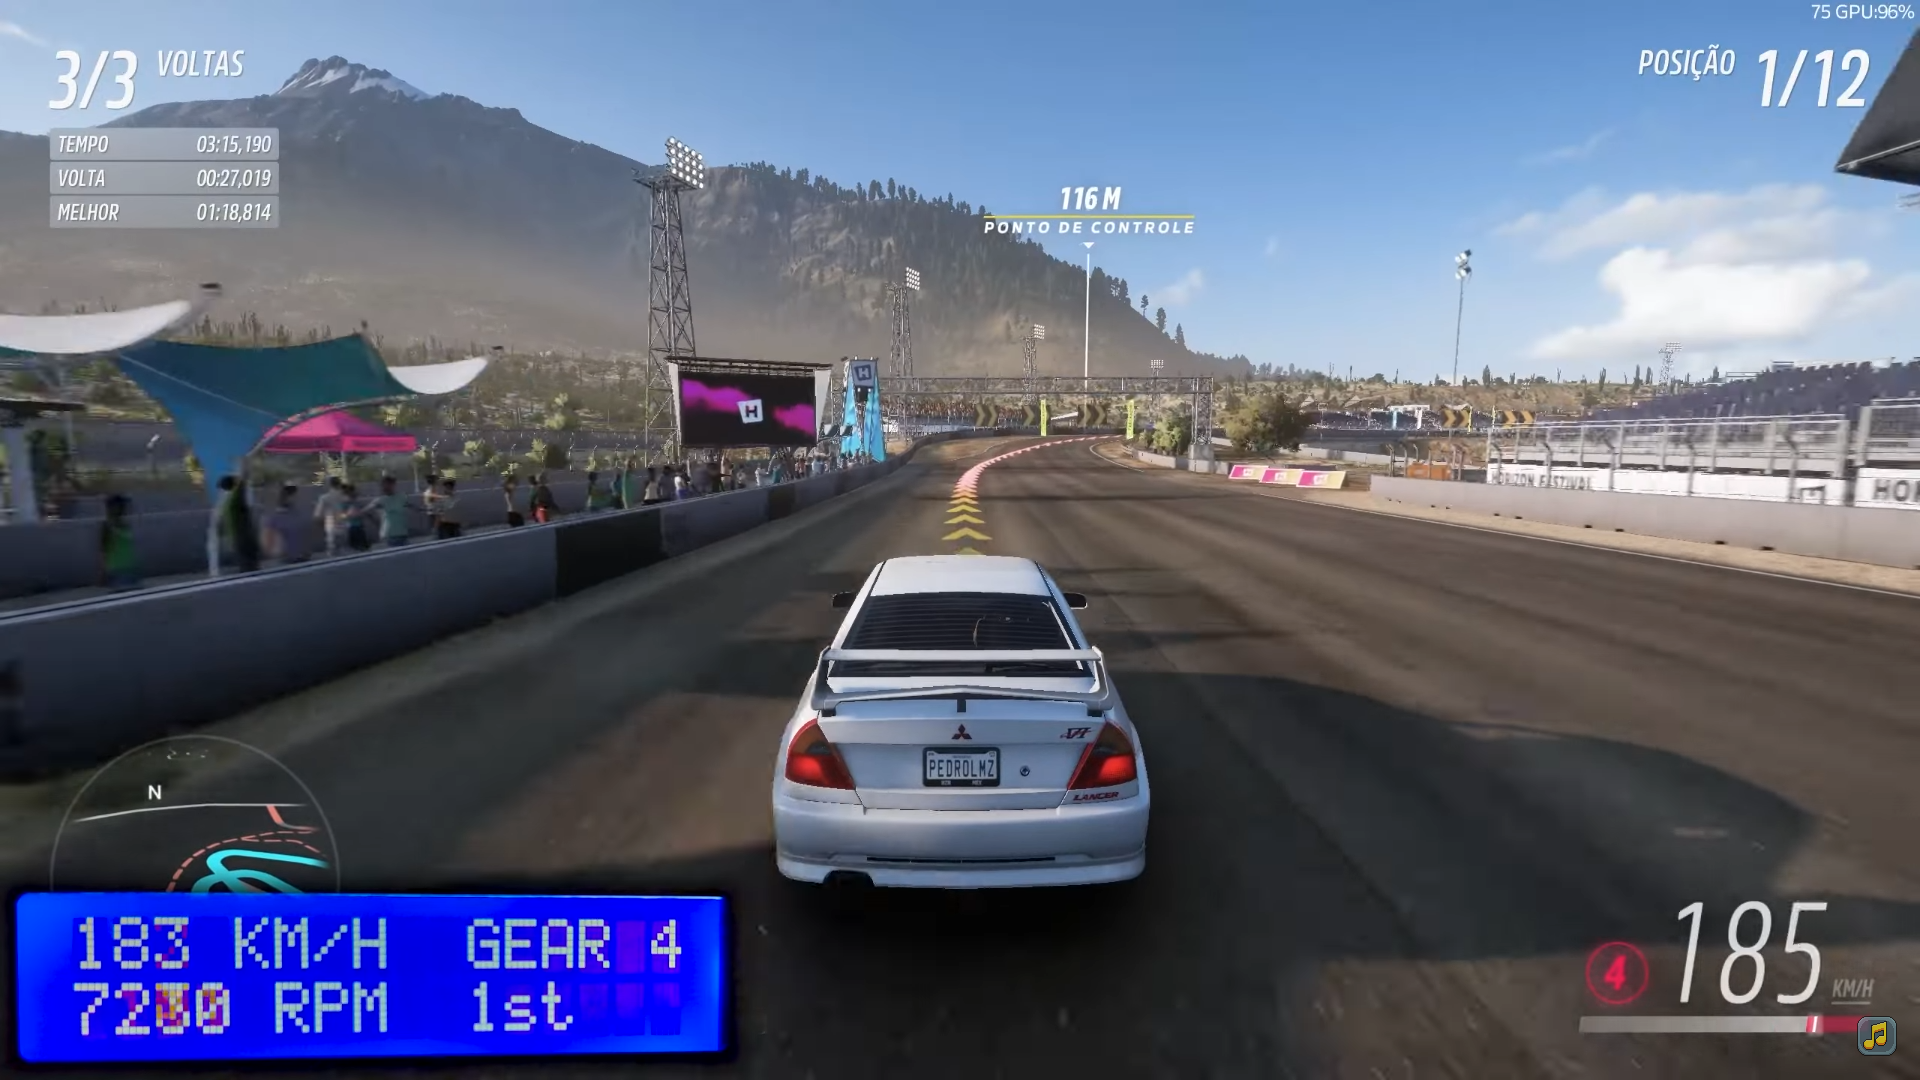
\includegraphics[width=.7\textwidth]{images/real_on_race.png}
  \caption{Exibição ao dirigir em uma corrida}
  \bigskip
  \label{fig:real_on_race}
  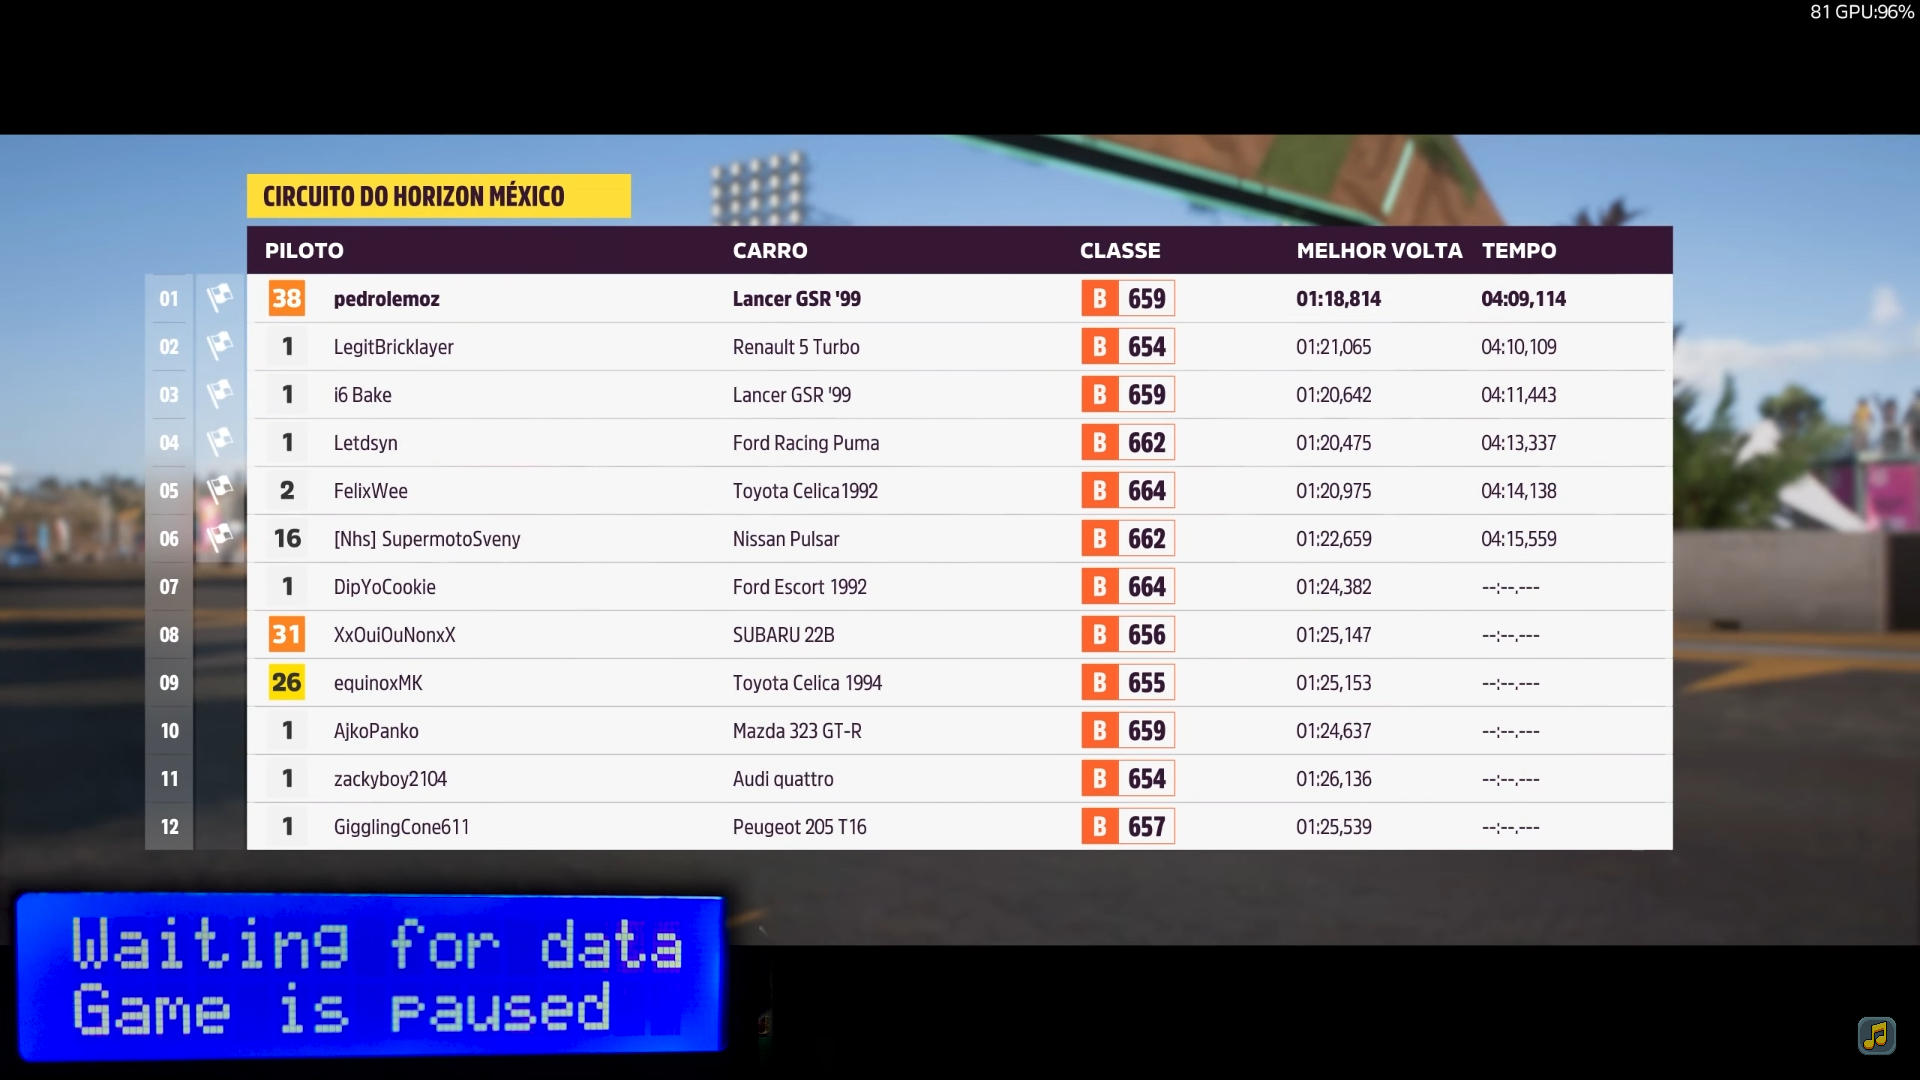
\includegraphics[width=.7\textwidth]{images/real_menu.png}
  \caption{Exibição em menus}
  \label{fig:real_menu}
\end{figure}

\clearpage

\section{Considerações finais}

Após concluir este projeto será possível compreender com mais clareza de que forma o microcontrolador
ESP32 é capaz de lidar com o protocolo UDP, bem como realizar a exibição de em um display 16x2 através do
protocolo I2C. Além disso, é possível verificar parcialmente como funciona a telemetria do jogo eletrônico
Forza Horizon 5.

Neste trabalho, verificou-se que existem algumas limitações principais na abordagem escolhida.
Por tratar-se de uma comunicação sem fios, existe um atraso entre os dados serem enviados pelo jogo e recebidos pelo microcontrolador.
Além disso, o ESP32 possui poucos recursos de hardware se comparado a um computador, que originalmente é o dispositivo alvo da telemetria.
Assim sendo, é necessário ter cautela quanto ao uso de memória e processamento ao se desenvolver para esta plataforma.

Em trabalhos futuros, pode ser investigada uma maneira de realizar o envio dos dados da telemetria por meio de um cabo, eliminando assim
o atraso que existe na implementação atual.
Ainda, os dados da telemetria poderiam ser decodificados pelo próprio computador que executa o jogo,
antes de serem enviados para o ESP32.

Existe ainda a possibilidade de periféricos serem criados para monitorar os dados da telemetria
de uma forma mais abrangente, armazenando os dados em bancos de dados, utilizando interfaces web,
e outros componentes, de forma a melhorar ainda mais a experiência por parte do utilizador.

\bibliographystyle{sbc}
\bibliography{sbc-template}

\end{document}
